%%%%%%%%%%%%%%%%%%%%%%%%%%%%%%%%%%%%%
%%%%%%%%%%%%%%%%%%%%%%%%%%%%%%%%%%%%%
\documentclass{article}

\usepackage[nonatbib]{neurips_2024}
\usepackage{fancyhdr}
\pagestyle{fancy}
\fancyhf{}
\usepackage[utf8]{inputenc} % allow utf-8 input
\usepackage[T1]{fontenc}    % use 8-bit T1 fonts
\usepackage{hyperref}       % hyperlinks
\usepackage{url}            % simple URL typesetting
\usepackage{booktabs}       % professional-quality tables
\usepackage{amsfonts}       % blackboard math symbols
\usepackage{nicefrac}       % compact symbols for 1/2, etc.
\usepackage{microtype}      % microtypography
\usepackage[table,dvipsnames]{xcolor}  % colors
\usepackage{siunitx}
\usepackage{amsmath}
\usepackage{amssymb}
\usepackage{csquotes}
\usepackage{enumitem}
\usepackage{ragged2e}
\usepackage{subcaption}
\usepackage{array}
\usepackage{caption}
\usepackage{tabularray}
\usepackage{titlesec}
\usepackage{chngcntr}
\usepackage{float}
\usepackage[most]{tcolorbox}
\usepackage[ruled,vlined,linesnumbered]{algorithm2e}

\definecolor{lightgray}{rgb}{0.95, 0.95, 0.95}

\newlist{arrowlist}{itemize}{1}
\setlist[arrowlist]{label=$\Rightarrow$}

\newcommand\smallcommentfont[1]{\footnotesize\ttfamily #1}

\newtcolorbox{coloredquote}[1][]{%
    % enhanced, breakable, 
    size=minimal,
    % frame hidden, 
    colframe=black!10!white, 
    colback=black!5!white,
    \texttt{#1}
}

%%%%%%%%%%%%%%%%%%%%%%%%%%%%%%%%%%%%%
\title{Course Project: Part 2\\
\vspace{2mm}
\small{Generative AI}
\\
\vspace{2mm}
\small{Saarland University -- Winter Semester 2024/25}
}

\author{%
  Martínez \\
  7057573 \\
  \texttt{cama00005@stud.uni-saarland.de} \\
}

\DeclareRobustCommand{\textitbf}[1]{\textbf{\textit{#1}}} % for bold italic text
\DeclareMathOperator*{\argmin}{arg\,min}
\DeclareMathOperator*{\argmax}{arg\,max}

% Remove default section number display
\titleformat{\section}
{\normalfont\large\bfseries}{}{0em}{}

% Redefine subsection formatting to remove bold
\titleformat{\subsection}
{\normalfont} % Format: normal font, large size
{\thesubsection}    % Label (e.g., (I.1))
{2em}               % Space between label and title
{}                  % Code before the title

% Make subsection counter global (not reset by sections)
\counterwithout{subsection}{section}

% Format subsection numbering as (I.1), (I.2), etc.
\renewcommand{\thesubsection}{(I.\arabic{subsection})}

\titlespacing*{\subsection}
  {0pt}{0.5\baselineskip}{0.01\baselineskip}

%%%%%%%%%%%%%%%%%%%%%%%%%%%%%%%%%%%%%
\begin{document}

\maketitle

%%%%%%%%%%%%%%%%%%%%%%%%%%%%%%%%%%%%%
% We consider several metrics to assess the overall performance of a model, including quality metrics for program repair and hint generation as well as usability metrics related to deployment in educational settings.

% \subsection*{Quality metrics for program repair}
% The quality of program repair will be evaluated using two metrics that focus on accuracy and efficiency. \textbf{RPass} (binary) examines whether the repaired program passes all test cases, signifying a successful fix. \textbf{REdit} (non-negative number) captures the token-level edit distance between the buggy and the repaired program, with a smaller edit distance reflecting that the repaired program is better aligned with the learner's buggy program. When reporting results, these metrics will be computed automatically.

% \subsection*{Quality metrics for hint generation}
% The quality of hint generation will be evaluated based on several binary metrics that define its pedagogical utility. \textbf{HCorrect} (binary) captures whether the generated hint provides correct information for resolving issues in the buggy program. \textbf{HInformative} (binary) captures whether the generated hint provides useful information to help the learner resolve bug(s). \textbf{HConceal} (binary) captures that the information in the generated hint is not too detailed, so the learner would also have to reason about implementing the fixes. \textbf{HComprehensible} (binary) captures whether the generated hint is easy to understand, presented in a readable format, and does not contain redundant information. We measure the overall quality of the generated hint by \textbf{HGood} (binary) that takes the value of 1 (good quality) when all the four attributes are rated as 1. When reporting results, these metrics would require manual annotations.

% \subsection*{Usability metrics}
% Beyond the quality metrics, there are several important usability metrics for deployment in educational settings, related to model size, user privacy aspects, and training/inference time. To account for these usability metrics, we will consider a small model Phi-3-mini and further load it as a 4-bit quantized version for inference/training. In Part\#2 of the project, we will explore parameter-efficient training (LoRA) and analyze the trade-offs between model quality and training efficiency. Here, we will use the metrics \textbf{TrainingTime} and \textbf{TrainingMemory} that capture the time and the memory used during the fine-tuning process.

\section{Part 2.a: Fine-tuning Baseline Models}\label{part-2a}

\vspace{-0.75\baselineskip}

% (I.11) Modify the parameters in the project_part2_evaluate.py script to generate program repairs using each of the two models (i.e., Phi-3-SFT-Repair-r16-alpha32 and Phi-3-SFT-Hints-r16-alpha32). Report RPass and REdit.

\textbf{(I.11)} Table \ref{I11:results} shows the comparison between the Phi-3-SFT-Repair-r16-alpha32 and Phi-3-SFT-Hints-r16-alpha32 models on the Repair task. As expected, the former is better on repair, than the latter, as demonstrated by the better values in both \emph{RPass} and \emph{REdit}, since it was specifically fine-tuned for the Repair task. The Phi-3-SFT-Hints-r16-alpha32 model, on the other hand, was fine-tuned for the hint generation task, and thus performs worse on the Repair task, but better on the Hint generation task, as \textbf{(I.12)} goes on to show.

% "repair_model": "project_part2_models/Phi-3-SFT-Hints_r16_alpha32",
% "RPass": 72.0,
% "REdit": 21.22222222222222,

% "repair_model": "project_part2_models/Phi-3-SFT-Repair_r16_alpha32",
% "RPass": 76.0,
% "REdit": 9.894736842105264,

\begin{table}[H]
    \caption{Program repair quality metrics, \emph{RPass} and \emph{REdit}, for the fine-tuned models on Repair and Hint tasks. In parentheses, the change in the metric compared to the Repair model is shown, where \textcolor{green}{green} means an improving change and \textcolor{red}{red} a worsening change. For \textbf{(I.11)}.}
    \vspace{0.5\baselineskip}
    \centering
    \begin{tblr}{
        colspec = {|Q[c,m]|Q[c,m]|Q[c,m]|},
        colsep=4pt,
        vlines,
        hlines,
        hspan=minimal,
        vspan=center,
        row{1} = {font=\bfseries}
        }
        Model                          & \textit{RPass} & \textit{REdit} \\
        \hline
        Phi-3-SFT-Hints\_r16\_alpha32  & $72.0$ (\textcolor{red}{$-4.0$}) & $21.22$ (\textcolor{red}{$+11.33$}) \\
        Phi-3-SFT-Repair\_r16\_alpha32 & $76.0$ (--) & $9.89$ (--) \\
    \end{tblr}
    \label{I11:results}
\end{table}

% (I.12) Modify the parameters in the project_part2_evaluate.py script to generate hints using each of the two models (i.e., Phi-3-SFT-Repair-r16-alpha32 and Phi-3-SFT-Hints-r16-alpha32). Evaluate the generated hints using the HGood metric [3] and report your results.

\textbf{(I.12)} Table \ref{I12:sft-repair-results} and \ref{I12:sft-hint-results} show the evaluation of the generated hints by the Phi-3-SFT-Repair-r16-alpha32 and Phi-3-SFT-Hints-r16-alpha32 models respectively using the \emph{HGood} metric \cite{HintsInBrowser2024}. As expected, since the Phi-3-SFT-Hints-r16-alpha32 model has been fine-tuned specifically on the Hint generation task, it performs very well on all metrics, achieving a score of $0.84$ in \emph{HGood}. On the other hand, the Phi-3-SFT-Repair-r16-alpha32 model, which has been fine-tuned on the Repair task, performs worse, with an average \emph{HGood} score of $0.2$. This model is only slightly better than the base Phi-3-mini model, which scored $0.16$ in \emph{HGood} in Project Part\#1.

\begin{table}[H]
    \caption{Hint Quality Metrics for Phi-3-SFT-Repair-r16-alpha32. This model is fine-tuned on Repair task. For \textbf{(I.12)}.}
    \vspace{0.5\baselineskip}
    \centering
    \begin{tblr}{
            colspec={X[0.3,c] X[0.2,c] X[0.2,c] X[0.3,c] X[0.2,c] X[0.4,c] X[0.15,c]},
            row{1}={font=\bfseries},
            colsep=4pt,
            row{even}={bg=gray!10},
            hlines,
            vlines,
            hspan=minimal,
            vspan=center,
        }
        Problem                   & Program & \textit{HCorrect}  & \textit{HInformative}  & \textit{HConceal} & \textit{HComprehensible} & \textit{HGood}  \\
        \hline
        \SetCell[r=5]{} Problem 1       & Prog. 1 & $1   $ & $1   $ & $0   $ & $1   $ & $0   $ \\
                                & Prog. 2 & $1   $ & $1   $ & $0   $ & $1   $ & $0   $ \\
                                & Prog. 3 & $1   $ & $1   $ & $1   $ & $1   $ & $1   $ \\
                                & Prog. 4 & $1   $ & $1   $ & $0   $ & $1   $ & $0   $ \\
                                & Prog. 5 & $1   $ & $0   $ & $0   $ & $1   $ & $0   $ \\
        \SetCell[c=2]{} Avg. Problem 1  &         & $1.0 $ & $0.8 $ & $0.2 $ & $1.0 $ & $0.2 $ \\
        \hline
        \SetCell[r=5]{} Problem 2       & Prog. 1 & $1   $ & $1   $ & $0   $ & $1   $ & $0   $ \\
                                & Prog. 2 & $0   $ & $0   $ & $1   $ & $1   $ & $0   $ \\
                                & Prog. 3 & $1   $ & $0   $ & $0   $ & $1   $ & $0   $ \\
                                & Prog. 4 & $0   $ & $0   $ & $1   $ & $1   $ & $0   $ \\
                                & Prog. 5 & $1   $ & $1   $ & $0   $ & $1   $ & $0   $ \\
        \SetCell[c=2]{} Avg. Problem 2  &         & $0.6 $ & $0.4 $ & $0.4 $ & $1.0 $ & $0.0 $ \\
        \hline
        \SetCell[r=5]{} Problem 3       & Prog. 1 & $1   $ & $1   $ & $0   $ & $1   $ & $0   $ \\
                                & Prog. 2 & $1   $ & $1   $ & $0   $ & $1   $ & $0   $ \\
                                & Prog. 3 & $1   $ & $1   $ & $1   $ & $1   $ & $1   $ \\
                                & Prog. 4 & $1   $ & $1   $ & $1   $ & $1   $ & $1   $ \\
                                & Prog. 5 & $1   $ & $1   $ & $0   $ & $1   $ & $0   $ \\
        \SetCell[c=2]{} Avg. Problem 3  &         & $1.0 $ & $1.0 $ & $0.4 $ & $1.0 $ & $0.4 $ \\
        \hline
        \SetCell[r=5]{} Problem 4       & Prog. 1 & $1   $ & $0   $ & $1   $ & $1   $ & $0   $ \\
                                & Prog. 2 & $1   $ & $0   $ & $0   $ & $1   $ & $0   $ \\
                                & Prog. 3 & $0   $ & $0   $ & $1   $ & $1   $ & $0   $ \\
                                & Prog. 4 & $0   $ & $0   $ & $1   $ & $1   $ & $0   $ \\
                                & Prog. 5 & $0   $ & $0   $ & $1   $ & $1   $ & $0   $ \\
        \SetCell[c=2]{} Avg. Problem 4  &         & $0.4 $ & $0.0 $ & $0.8 $ & $1.0 $ & $0.0 $ \\
        \hline
        \SetCell[r=5]{} Problem 5       & Prog. 1 & $1   $ & $1   $ & $0   $ & $1   $ & $0   $ \\
                                & Prog. 2 & $1   $ & $1   $ & $1   $ & $1   $ & $1   $ \\
                                & Prog. 3 & $0   $ & $0   $ & $0   $ & $1   $ & $0   $ \\
                                & Prog. 4 & $1   $ & $1   $ & $0   $ & $1   $ & $0   $ \\
                                & Prog. 5 & $1   $ & $1   $ & $1   $ & $1   $ & $1   $ \\
        \SetCell[c=2]{} Avg. Problem 5  &         & $0.8 $ & $0.8 $ & $0.4 $ & $1.0 $ & $0.4 $ \\
        \hline
        \SetCell[c=2]{} Overall Average &         & $0.76$ & $0.6$ & $0.44$ & $1.0$  & $0.2$
    \end{tblr}
    \label{I12:sft-repair-results}
\end{table}

\begin{table}[H]
    \caption{Hint Quality Metrics for Phi-3-SFT-Hints-r16-alpha32. This model is fine-tuned on Hint generation. For \textbf{(I.12)}.}
    \vspace{0.5\baselineskip}
    \centering
    \begin{tblr}{
            colspec={X[0.3,c] X[0.2,c] X[0.2,c] X[0.3,c] X[0.2,c] X[0.4,c] X[0.15,c]},
            row{1}={font=\bfseries},
            colsep=4pt,
            row{even}={bg=gray!10},
            hlines,
            vlines,
            hspan=minimal,
            vspan=center,
        }
        Problem                   & Program & \textit{HCorrect}  & \textit{HInformative}  & \textit{HConceal} & \textit{HComprehensible} & \textit{HGood}  \\
        \hline
        \SetCell[r=5]{} Problem 1       & Prog. 1 & $1  $ & $1   $ & $1   $ & $1  $ & $1$   \\
                                & Prog. 2 & $1  $ & $1   $ & $1   $ & $1  $ & $1$   \\
                                & Prog. 3 & $1  $ & $1   $ & $1   $ & $1  $ & $1$   \\
                                & Prog. 4 & $1  $ & $0   $ & $1   $ & $1  $ & $0$   \\
                                & Prog. 5 & $1  $ & $1   $ & $1   $ & $1  $ & $1$   \\
        \SetCell[c=2]{} Avg. Problem 1  &         & $1.0$ & $0.8 $ & $1.0 $ & $1.0$ & $0.8$ \\
        \hline
        \SetCell[r=5]{} Problem 2       & Prog. 1 & $1  $ & $1   $ & $1   $ & $1  $ & $1$   \\
                                & Prog. 2 & $1  $ & $1   $ & $1   $ & $1  $ & $1$   \\
                                & Prog. 3 & $1  $ & $1   $ & $1   $ & $1  $ & $1$   \\
                                & Prog. 4 & $1  $ & $1   $ & $1   $ & $1  $ & $1$   \\
                                & Prog. 5 & $1  $ & $0   $ & $1   $ & $1  $ & $0$   \\
        \SetCell[c=2]{} Avg. Problem 2  &         & $1.0$ & $0.8 $ & $1.0 $ & $1.0$ & $0.8$ \\
        \hline
        \SetCell[r=5]{} Problem 3       & Prog. 1 & $1  $ & $1   $ & $1   $ & $1  $ & $1$   \\
                                & Prog. 2 & $1  $ & $0   $ & $1   $ & $1  $ & $0$   \\
                                & Prog. 3 & $1  $ & $1   $ & $1   $ & $1  $ & $1$   \\
                                & Prog. 4 & $1  $ & $1   $ & $1   $ & $1  $ & $1$   \\
                                & Prog. 5 & $1  $ & $1   $ & $1   $ & $1  $ & $1$   \\
        \SetCell[c=2]{} Avg. Problem 3  &         & $1.0$ & $0.8 $ & $1.0 $ & $1.0$ & $0.8$ \\
        \hline
        \SetCell[r=5]{} Problem 4       & Prog. 1 & $0  $ & $0   $ & $1   $ & $1  $ & $0$  \\
                                & Prog. 2 & $1  $ & $1   $ & $1   $ & $1  $ & $1$   \\
                                & Prog. 3 & $1  $ & $1   $ & $1   $ & $1  $ & $1$   \\
                                & Prog. 4 & $1  $ & $1   $ & $1   $ & $1  $ & $1$   \\
                                & Prog. 5 & $1  $ & $1   $ & $1   $ & $1  $ & $1$   \\
        \SetCell[c=2]{} Avg. Problem 4  &         & $0.8$ & $0.8 $ & $1.0 $ & $1.0$ & $0.8$ \\
        \hline
        \SetCell[r=5]{} Problem 5       & Prog. 1 & $1  $ & $1   $ & $1   $ & $1  $ & $1$   \\
                                & Prog. 2 & $1  $ & $1   $ & $1   $ & $1  $ & $1$   \\
                                & Prog. 3 & $1  $ & $1   $ & $1   $ & $1  $ & $1$   \\
                                & Prog. 4 & $1  $ & $1   $ & $1   $ & $1  $ & $1$   \\
                                & Prog. 5 & $1  $ & $1   $ & $1   $ & $1  $ & $1$   \\
        \SetCell[c=2]{} Avg. Problem 5  &         & $1.0$ & $1.0 $ & $1.0 $ & $1.0$ & $1.0$ \\
        \hline
        \SetCell[c=2]{} Overall Average &         & $0.96$ & $0.84$ & $1.0$ & $1.0$  & $0.84$
    \end{tblr}
    \label{I12:sft-hint-results}
\end{table}

\section{Part 2.b: Fine-tuning for Program Repair with Varying LoRA Parameters}\label{part-2b}

% (I.13) Evaluate the three different fine-tuned models with varying (r, α) on program repair. Report program repair quality metrics (RPass, REdit), TrainingTime, and TrainingMemory. In terms of quality metrics, compare the results of different fine-tuned models with those of the base Phi-3-mini in I.3 of Project Part#1.

% "repair_model": "project_part2_models/Phi-3-SFT-Repair_r4_alpha8",
% "RPass": 60.0,
% "REdit": 11.466666666666667,

% "repair_model": "project_part2_models/Phi-3-SFT-Repair_r16_alpha32",
% "RPass": 76.0,
% "REdit": 9.894736842105264,

% "repair_model": "project_part2_models/Phi-3-SFT-Repair_r64_alpha128",
% "RPass": 84.0,
% "REdit": 17.142857142857142,

\textbf{(I.13)} Table \ref{I13:results} shows a comparison between different fine-tuned versions of the Phi-3-mini model on the Repair task using varying LoRA parameters. Recall that in Project Part\#1 (see Table \ref{appendix-I3-results} in \hyperref[appendix:I3-results]{\textbf{Appendix}}), the base Phi-3-mini scored $36.0$ in \emph{RPass} and $18.11$ in \emph{REdit}, which is significantly worse than any of the fine-tuned models. This means that the fine-tuning process with LoRA was effective and greatly improved the model's performance on the Repair task.

\begin{table}[H]
    \caption{Program repair quality metrics, \emph{RPass} and \emph{REdit}, for the fine-tuned models on Repair task using different LoRA
    parameter configurations: $(r, \alpha) = {(4, 8), (16, 32), (64, 128)}$. In parentheses, the change in the metric compared to a base configuration, chosen to be $(16, 32)$, is shown, where \textcolor{green}{green} means an improving change and \textcolor{red}{red} a worsening change. For \textbf{(I.13)}.}
    \vspace{0.5\baselineskip}
    \centering
    \begin{tblr}{
        colspec = {|Q[c,m]|Q[c,m]|Q[c,m]|},
        colsep=4pt,
        vlines,
        hlines,
        hspan=minimal,
        vspan=center,
        row{1} = {font=\bfseries}
        }
        \boldmath$(r, \alpha)$ & \textit{RPass}                      & \textit{REdit}                     \\
        \hline
        $(4, 8)$               & $60.0$ (\textcolor{red}{$-16.0$})                         & $11.47$ (\textcolor{red}{$+1.58$}) \\
        $(16, 32)$             & $76.0$ (--) & $9.89$ (--)                        \\
        $(64, 128)$            & $84.0$ (\textcolor{green}{$+8.0$}) & $17.14$ (\textcolor{red}{$+7.25$}) \\
    \end{tblr}
    \label{I13:results}
\end{table}

\begin{figure}[h]
    \centering
    \begin{subfigure}{0.45\textwidth}
        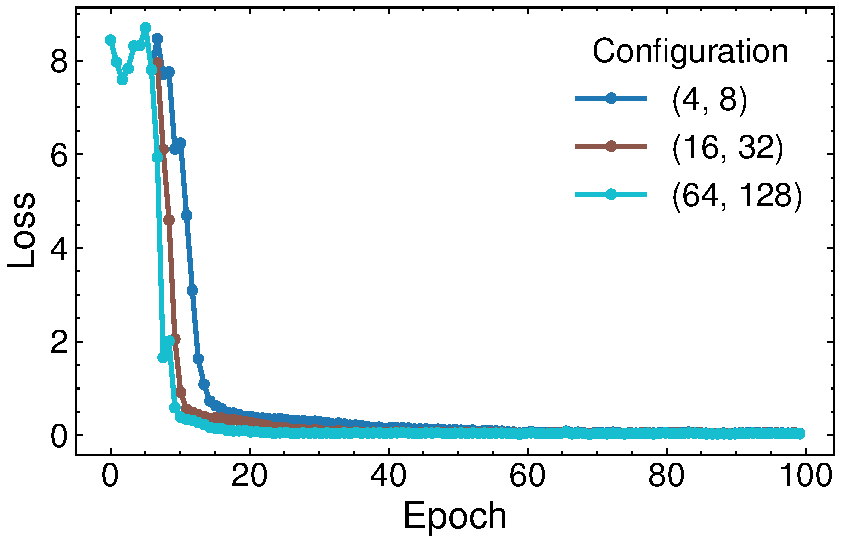
\includegraphics[width=0.9\linewidth]{../images/I.14 Results_loss.pdf}
        \caption{Loss over training epochs. \vspace{3.5mm}}
    \end{subfigure}
    \hfill
    \begin{subfigure}{0.45\textwidth}
        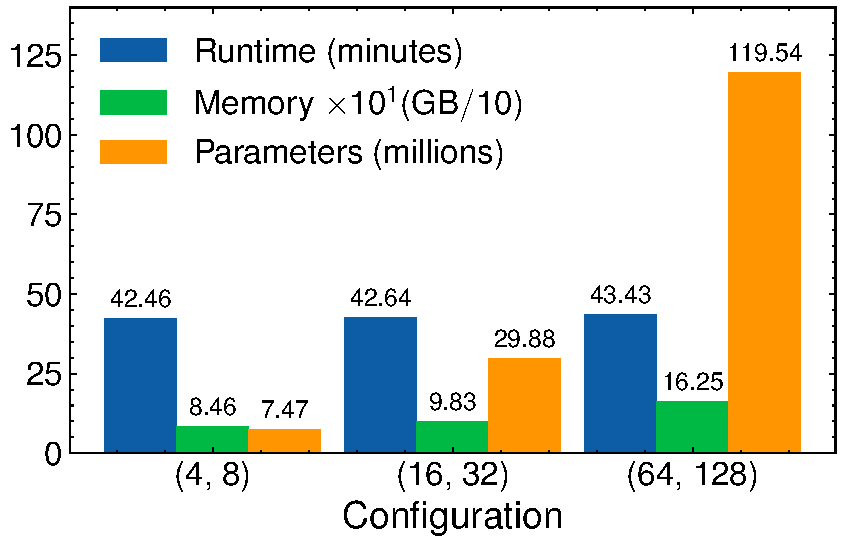
\includegraphics[width=0.9\linewidth]{../images/I.14 Results_metrics.pdf}
        \caption{\emph{TrainingTime}, \emph{TrainingMemory} and number of trained parameters comparison.}
    \end{subfigure}
    \caption{Trade-offs between LoRA parameter configurations in terms of loss evolution, \emph{TrainingTime}, \emph{TrainingMemory}, and number of trained parameters. These experiments were conducted with a GPU T4 instance on \href{https://colab.research.google.com/}{Google Colab}. For \textbf{(I.13)}.}
    \label{fig:I13-results-plots}
\end{figure}

% (I.14) Analyze the tradeoffs between LoRA parameter configurations in terms of program repair quality and TrainingMemory. Include a discussion about the TrainingMemory and the number of trained parameters for each configuration (printed in the console when starting training).

\textbf{(I.14)} Figure \ref{fig:I13-results-plots} shows that the \emph{TrainingTime} of all three LoRA configurations are very similar. The main difference thus lies in the \emph{TrainingMemory} and the number of trained parameters. Naturally, the $(64, 128)$ configuration has the highest \emph{TrainingMemory} and number of trained parameters, which is expected given the higher values of $r$ and $\alpha$. More precisely, the number of trained parameters increases approximately by a factor of $4$ when going from $(4, 8)$ to $(16, 32)$, and by a factor of $4$ again when going from $(16, 32)$ to $(64, 128)$. This is consistent with the theoretical analysis of LoRA, which predicts that the number of parameters scales quadratically with the values of $r$ and $\alpha$ \cite{LoRA2021}. 

On the other hand, the increase of \emph{TrainingMemory} between configurations is not as extreme. From $(4, 8)$ to $(16, 32)$, there is a $16$\% increase, and from $(16, 32)$ to $(64, 128)$, there is a $65$\% increase. This is likely due to the fact that the memory requirements of the model are not only determined by the number of parameters, but also by the size of the intermediate activations and the gradients during training.

Finally, in terms of program repair quality, the $(64, 128)$ configuration outperforms the other two configurations in terms of \emph{RPass}, but has the highest \emph{REdit}, suggesting that it might be overfitting to the training data. The $(4, 8)$ configuration has the lowest \emph{RPass} and the second highest \emph{REdit}, indicating that it is underfitting. The $(16, 32)$ configuration is a good balance between the two, achieving a value of \emph{RPass} only 8 points lower than the best, but at the same time the lowest \emph{REdit}. 

The choice between the three configurations will depend on the specific requirements of the application. Personally, in the feedback generation domain, the $(16, 32)$ configuration would be the most suitable, as it can generate accurate repairs (high \emph{RPass}) with the lowest number of changes to the buggy code compared to the other models (low \emph{REdit}). This allows a student to learn from the generated feedback without being overwhelmed by too many changes or dissapointed that the complete idea of the code was changed.

\section{Part 2.c: Fine-tuning on Merged Datasets}\label{part-2c}

% (I.15) Evaluate the multi-task model on program repair. Report results based on the program repair quality metrics as done in I.11.

\textbf{(I.15)} Table \ref{I15:results} shows the comparison between the Phi-3-SFT-Repair-r16-alpha32, Phi-3-SFT-Hints-r16-alpha32 and Phi-3-SFT-Merged-r16-alpha32 models on the Repair task. The latter, fine-tuned on both Repair and Hint tasks outperforms the other two in terms of \emph{RPass} and achieves the second lowest \emph{REdit}. This suggests that the multi-task learning approach is effective in improving the model's performance on the Repair task, at the cost of being slightly less conservative in suggesting changes to the student's buggy code.

% "repair_model": "project_part2_models/Phi-3-SFT-Repair_r16_alpha32_combined",
% "RPass": 80.0,
% "REdit": 14.6,

\begin{table}[H]
    \caption{Program repair quality metrics, \emph{RPass} and \emph{REdit}, for the fine-tuned models on Repair, Hint and both tasks combined. In parentheses, the change in the metrics compared to the multi-task model (Phi-3-SFT-Merged\_r16\_alpha32) is shown, where \textcolor{green}{green} means an improving change and \textcolor{red}{red} a worsening change. The results of \textbf{(I.11)} are included for ease of comparison. For \textbf{(I.15)}.}
    \vspace{0.5\baselineskip}
    \centering
    \begin{tblr}{
        colspec = {|Q[c,m]|Q[c,m]|Q[c,m]|},
        colsep=4pt,
        vlines,
        hlines,
        hspan=minimal,
        vspan=center,
        row{1} = {font=\bfseries}
        }
        Model                          & \textit{RPass} & \textit{REdit} \\
        \hline
        Phi-3-SFT-Hints\_r16\_alpha32  & $72.0$ (\textcolor{red}{$-8.0$}) & $21.22$ (\textcolor{red}{$+6.62$}) \\
        Phi-3-SFT-Repair\_r16\_alpha32 & $76.0$ (\textcolor{red}{$-4.0$}) & $9.89$ (\textcolor{green}{$-4.71$}) \\
        Phi-3-SFT-Merged\_r16\_alpha32 & $80.0$ (--) & $14.6$ (--) \\
    \end{tblr}
    \label{I15:results}
\end{table}

% (I.16) Evaluate the multi-task model on hint generation. Report results based on the hint generation quality metrics as done in I.12.

\textbf{(I.16)} Table \ref{I16:sft-merged-results} shows the evaluation of the Phi-3-SFT-Merged-r16-alpha32 model on the Hint generation task using the \emph{HGood} metric \cite{HintsInBrowser2024}. As expected, the model performs very well on all metrics, achieving a score of $0.92$ in \emph{HGood}. Given the results of \textbf{(I.15)}, this means that this model became the best at both tasks, at the same time.

This multi-task learning approach of using a concatenation of both datasets (Repair + Hint) offered a more diverse scenario for a model to learn from. Both of these tasks intuitively benefit from one another. During training, the model is given access to the repairs of the buggy programs, which should give it exact guidelines on what to hint at for a student. Thus a diverse dataset such as this one contributes to a hand-in-hand improvement in the model's performance on both tasks.

Finally, a comparison of all evaluated Phi-3-mini models is provided with Figure \ref{fig:I.16-results}, in order to see how the SFT models fare against the base model and the CoT model from Project Part\#1.

\begin{figure}[h]
    \centering
    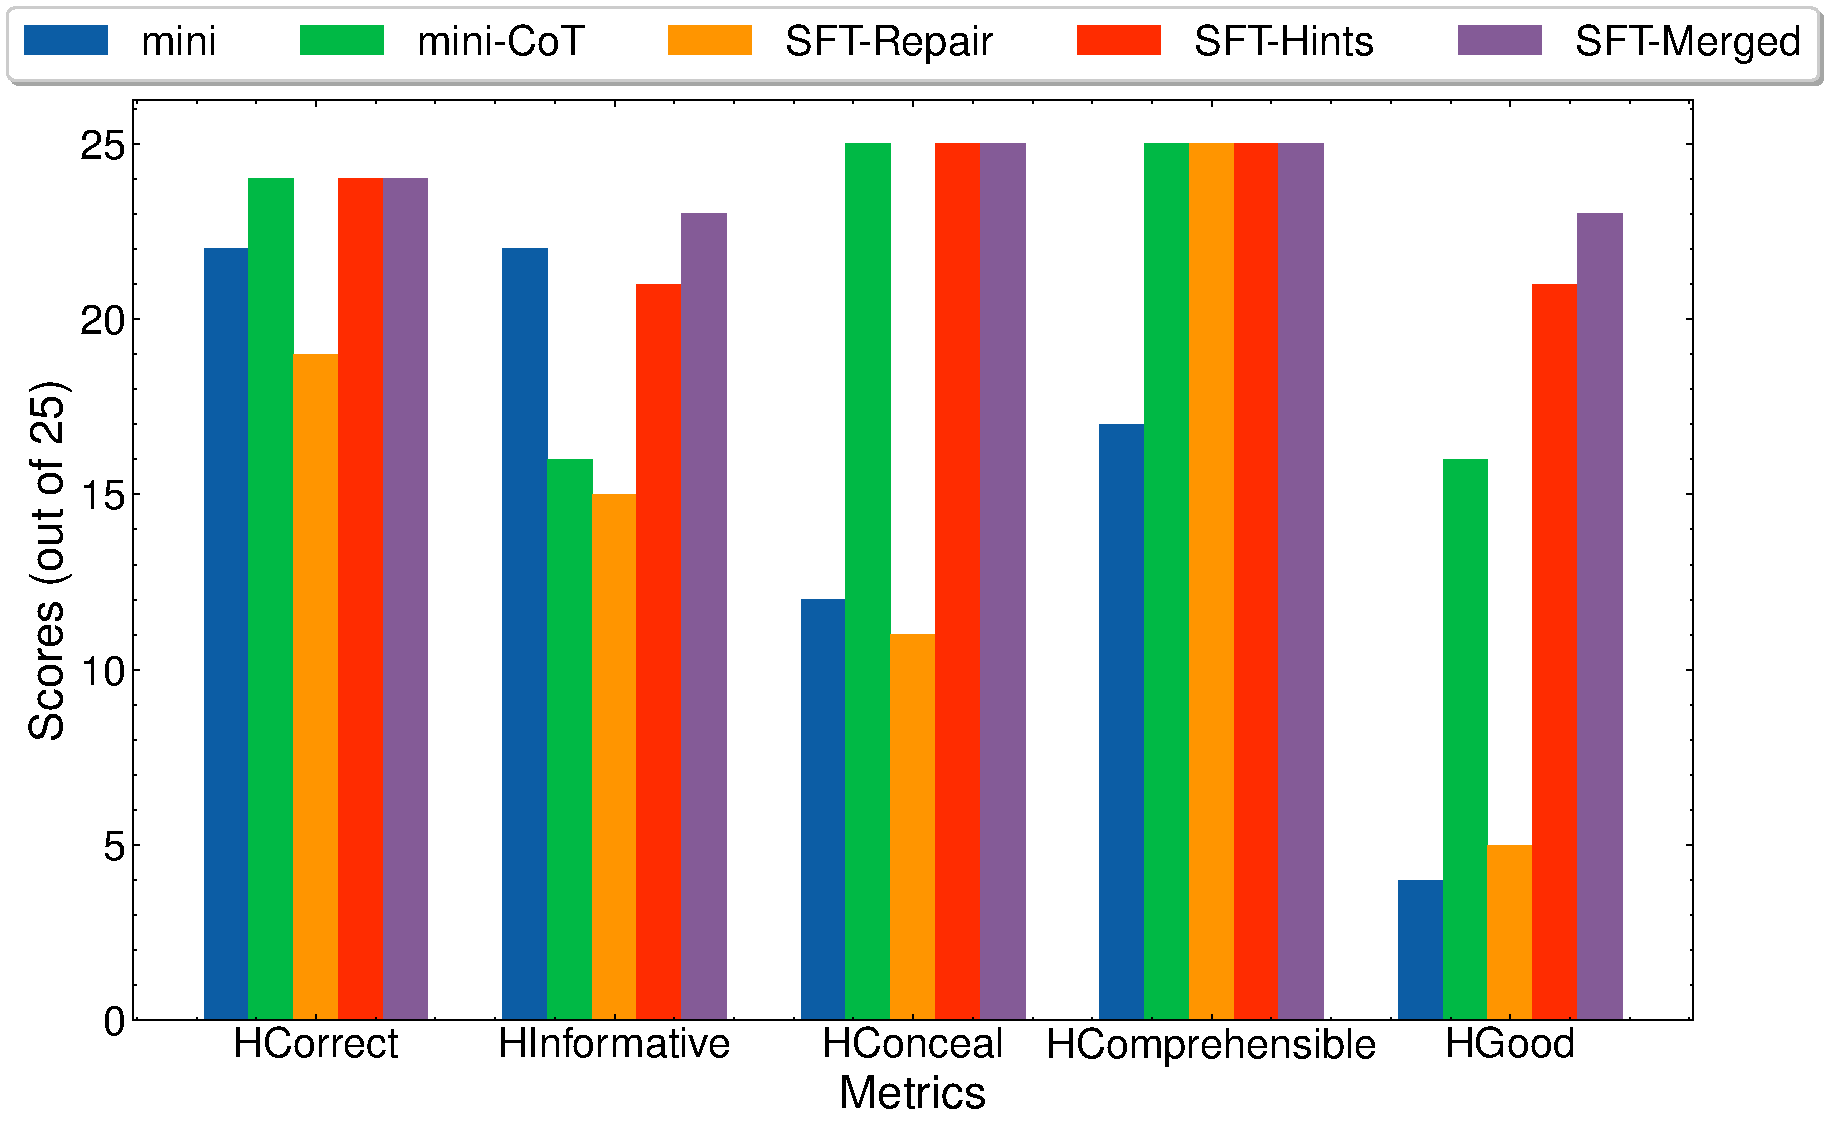
\includegraphics[width=0.9\linewidth]{../images/all_models_hint_metrics_plot.pdf}
    \caption{Comparison between all Phi-3-mini models: the base model, with CoT (both from Project Part\#1), Phi-3-SFT-Repair-r16-alpha32, Phi-3-SFT-Hints-r16-alpha32 and Phi-3-SFT-Merged-r16-alpha32 models, evaluated on the Hint generation task in terms of the \emph{HGood} metric. For \textbf{(I.16)}.}
    \label{fig:I.16-results}
\end{figure}

\begin{table}[H]
    \caption{Hint Quality Metrics for Phi-3-SFT-Merged-r16-alpha32. This model is fine-tuned on both Repair and Hint tasks. For \textbf{(I.16)}.}
    \vspace{0.5\baselineskip}
    \centering
    \begin{tblr}{
            colspec={X[0.3,c] X[0.2,c] X[0.2,c] X[0.3,c] X[0.2,c] X[0.4,c] X[0.15,c]},
            row{1}={font=\bfseries},
            colsep=4pt,
            row{even}={bg=gray!10},
            hlines,
            vlines,
            hspan=minimal,
            vspan=center,
        }
        Problem                   & Program & \textit{HCorrect}  & \textit{HInformative}  & \textit{HConceal} & \textit{HComprehensible} & \textit{HGood}  \\
        \hline
        \SetCell[r=5]{} Problem 1       & Prog. 1 & $1   $ & $1   $ & $1   $ & $1   $ & $1   $ \\
                                & Prog. 2 & $1   $ & $1   $ & $1   $ & $1   $ & $1   $ \\
                                & Prog. 3 & $1   $ & $1   $ & $1   $ & $1   $ & $1   $ \\
                                & Prog. 4 & $1   $ & $1   $ & $1   $ & $1   $ & $1   $ \\
                                & Prog. 5 & $1   $ & $1   $ & $1   $ & $1   $ & $1   $ \\
        \SetCell[c=2]{} Avg. Problem 1  &         & $1.0 $ & $1.0 $ & $1.0 $ & $1.0 $ & $1.0 $ \\
        \hline
        \SetCell[r=5]{} Problem 2       & Prog. 1 & $1   $ & $1   $ & $1   $ & $1   $ & $1   $ \\
                                & Prog. 2 & $1   $ & $1   $ & $1   $ & $1   $ & $1   $ \\
                                & Prog. 3 & $1   $ & $1   $ & $1   $ & $1   $ & $1   $ \\
                                & Prog. 4 & $1   $ & $1   $ & $1   $ & $1   $ & $1   $ \\
                                & Prog. 5 & $1   $ & $1   $ & $1   $ & $1   $ & $1   $ \\
        \SetCell[c=2]{} Avg. Problem 2  &         & $1.0 $ & $1.0 $ & $1.0 $ & $1.0 $ & $1.0 $ \\
        \hline
        \SetCell[r=5]{} Problem 3       & Prog. 1 & $1   $ & $1   $ & $1   $ & $1   $ & $1   $ \\
                                & Prog. 2 & $1   $ & $1   $ & $1   $ & $1   $ & $1   $ \\
                                & Prog. 3 & $1   $ & $1   $ & $1   $ & $1   $ & $1   $ \\
                                & Prog. 4 & $1   $ & $1   $ & $1   $ & $1   $ & $1   $ \\
                                & Prog. 5 & $1   $ & $1   $ & $1   $ & $1   $ & $1   $ \\
        \SetCell[c=2]{} Avg. Problem 3  &         & $1.0 $ & $1.0 $ & $1.0 $ & $1.0 $ & $1.0 $ \\
        \hline
        \SetCell[r=5]{} Problem 4       & Prog. 1 & $1   $ & $1   $ & $1   $ & $1   $ & $1   $ \\
                                & Prog. 2 & $1   $ & $1   $ & $1   $ & $1   $ & $1   $ \\
                                & Prog. 3 & $1   $ & $1   $ & $1   $ & $1   $ & $1   $ \\
                                & Prog. 4 & $0   $ & $0   $ & $1   $ & $1   $ & $0   $ \\
                                & Prog. 5 & $1   $ & $1   $ & $1   $ & $1   $ & $1   $ \\
        \SetCell[c=2]{} Avg. Problem 4  &         & $0.8 $ & $0.8 $ & $1.0 $ & $1.0 $ & $0.8 $ \\
        \hline
        \SetCell[r=5]{} Problem 5       & Prog. 1 & $1   $ & $1   $ & $1   $ & $1   $ & $1   $ \\
                                & Prog. 2 & $1   $ & $1   $ & $1   $ & $1   $ & $1   $ \\
                                & Prog. 3 & $1   $ & $0   $ & $1   $ & $1   $ & $0   $ \\
                                & Prog. 4 & $1   $ & $1   $ & $1   $ & $1   $ & $1   $ \\
                                & Prog. 5 & $1   $ & $1   $ & $1   $ & $1   $ & $1   $ \\
        \SetCell[c=2]{} Avg. Problem 5  &         & $1.0 $ & $0.8 $ & $1.0 $ & $1.0 $ & $0.8 $ \\
        \hline
        \SetCell[c=2]{} Overall Average &         & $0.96$ & $0.92$ & $1.0$ & $1.0$  & $0.92$
    \end{tblr}
    \label{I16:sft-merged-results}
\end{table}

% (I.17) Report and analyze the performance w.r.t. TrainingTime and TrainingMemory. Explain the approach you used to create the dataset and fine-tune the multi-task model, noting challenges and key observations. Discuss the performance changes compared to specialized models in Part 2.a and the possible reasons behind them.

\textbf{(I.17)} In order to create the merged dataset to train the multi-task model (Phi-3-SFT-Merged\_r16\_alpha32), I added a simple concatenation of both datasets (Repair + Hint) in \texttt{project\_part2\_assemble\_dataset.py} and a shuffling of the result afterwards. 

Figure \ref{fig:I.17-results} shows the trade-offs between the specialized models and the multi-task model in terms of loss evolution, \emph{TrainingTime}, \emph{TrainingMemory}, and number of trained parameters. The multi-task model with $(r, \alpha) = (16, 32)$ has a higher \emph{TrainingTime}, but suprisingly has a better loss evolution compared to the specialized models. That is, the loss decreases rapidly in the first few epochs, indicating rapid learning, and then plateaus similar to the other models. 

On the other hand, the \emph{TrainingMemory} between the specialized model for the Repair task and the multi-task model is the same.

\begin{figure}[h]
    \centering
    \begin{subfigure}{0.45\textwidth}
        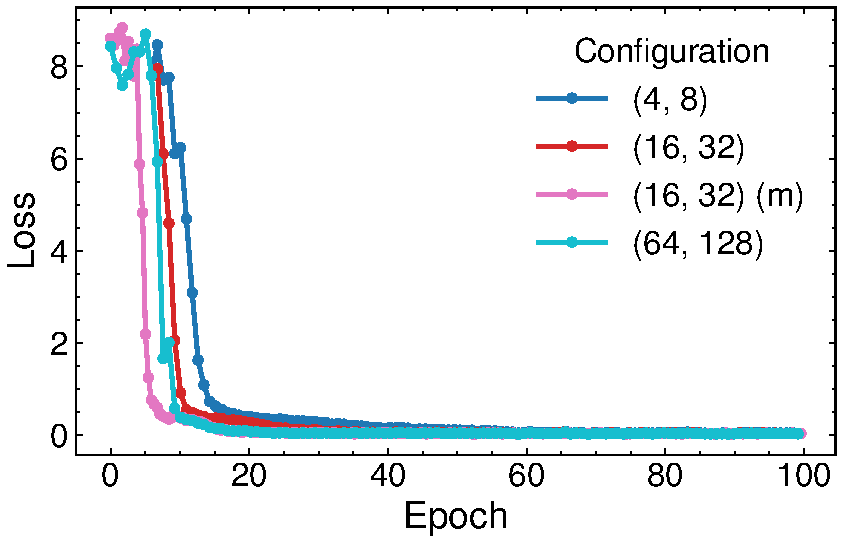
\includegraphics[width=0.9\linewidth]{../images/I.17 Results_loss.pdf}
        \caption{Loss over training epochs. \vspace{3.5mm}}
    \end{subfigure}
    \hfill
    \begin{subfigure}{0.45\textwidth}
        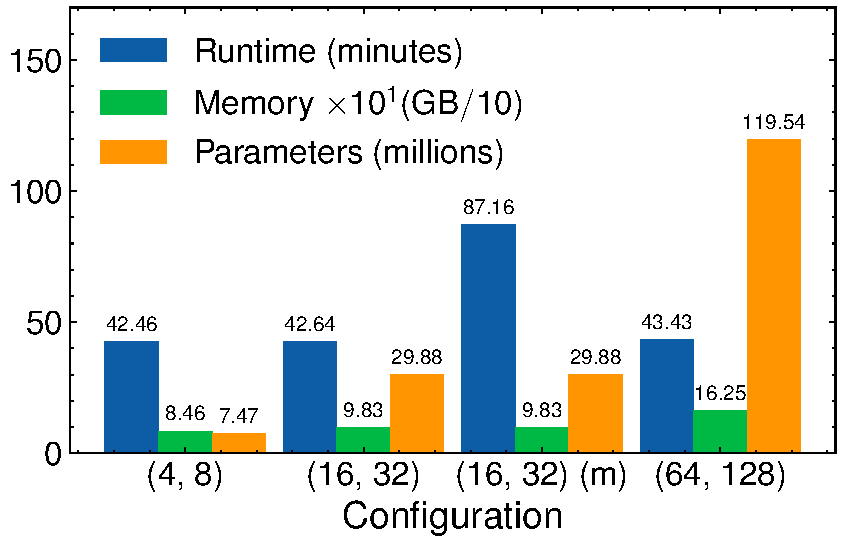
\includegraphics[width=0.9\linewidth]{../images/I.17 Results_metrics.pdf}
        \caption{\emph{TrainingTime}, \emph{TrainingMemory} and number of trained parameters comparison.}
    \end{subfigure}
    \caption{Trade-offs between the specialized models and the multi-task model in terms of loss evolution, \emph{TrainingTime}, \emph{TrainingMemory}, and number of trained parameters. The (m) indicates the multi-task model. These experiments were conducted with a GPU T4 instance on \href{https://colab.research.google.com/}{Google Colab}. For \textbf{(I.17)}.}
    \label{fig:I.17-results}
\end{figure}

As expected, the $(4, 8)$ configuration has the lowest number of parameters and thus incurs in the least \emph{TrainingMemory}. The \emph{TrainingTime} between all configurations, $(4, 8)$, $(16, 32)$ and $(64, 128)$ is the same, which is also supported by the loss evolution plot. This means that the model does not gain anything from adding $4\times$ more parameters, going from $(16, 32)$ to $(64, 128)$, as their loss curve almost overlap. And if we look at Table \ref{I15:results} again, the gain in \emph{RPass} is only $4$ points better than $(16, 32)$, but the \emph{REdit} is worse. On the other hand, the $(16, 32)$ (m) configuration has approximately $2\times$ the \emph{TrainingTime} than all the others, which is expected as the dataset grew in size.

Therefore, the $(16, 32)$ configuration seems to be the best trade-off between the number of parameters, \emph{TrainingMemory}, and the loss evolution. It has a good balance between the number of parameters and \emph{TrainingMemory}, and the results from Table \ref{I15:results} shows that it is not overfitting as $(64, 128)$.

Figure \ref{fig:I.17-A100-results} shows the same concepts, as Figure \ref{fig:I.17-results}, but for a GPU A100 instance. Using this GPU significantly reduced the \emph{TrainingTime} for all models, especially for the multi-task model. Nevertheless, if we take into account relative performance, the multi-task model still requires $2\times$ the \emph{TrainingTime} of the specialized model for the Repair task, i.e., $6.63$ minutes vs. $13.50$ minutes with an A100 and $42.64$ minutes vs $87.16$ minutes with a T4, respectively.

On the other hand, the loss over training epochs showcase the \emph{scaling laws}, as we learned in Week 4. All models showcase a stepper and smoother decrease in loss as the number of epochs increases. That is, a higher computing power effectively reduced the time to reach a certain loss value, eventhough the hyperparameters, model architecture and datasets were the same \cite{scalinglaws2020}.

\begin{figure}[h]
    \centering
    \begin{subfigure}{0.45\textwidth}
        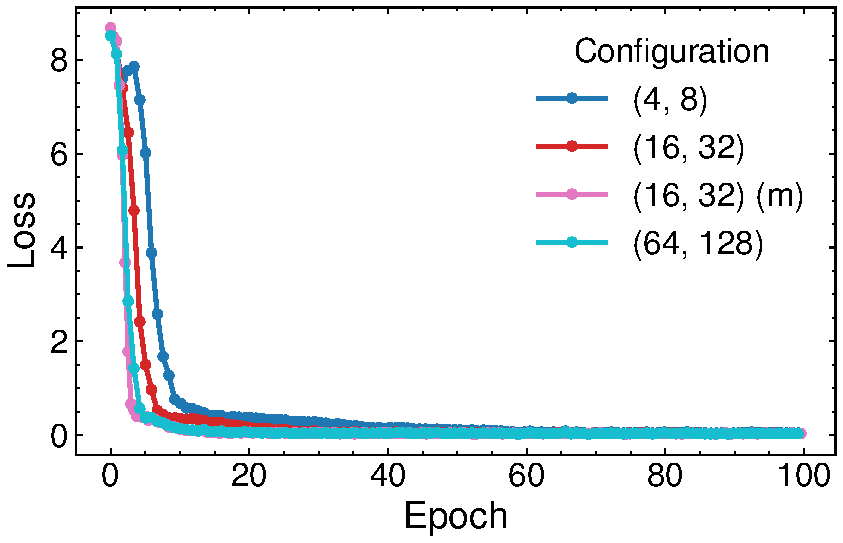
\includegraphics[width=0.9\linewidth]{../images/I.17 Results_A100_loss.pdf}
        \caption{Loss over training epochs. \vspace{3.5mm}}
    \end{subfigure}
    \hfill
    \begin{subfigure}{0.45\textwidth}
        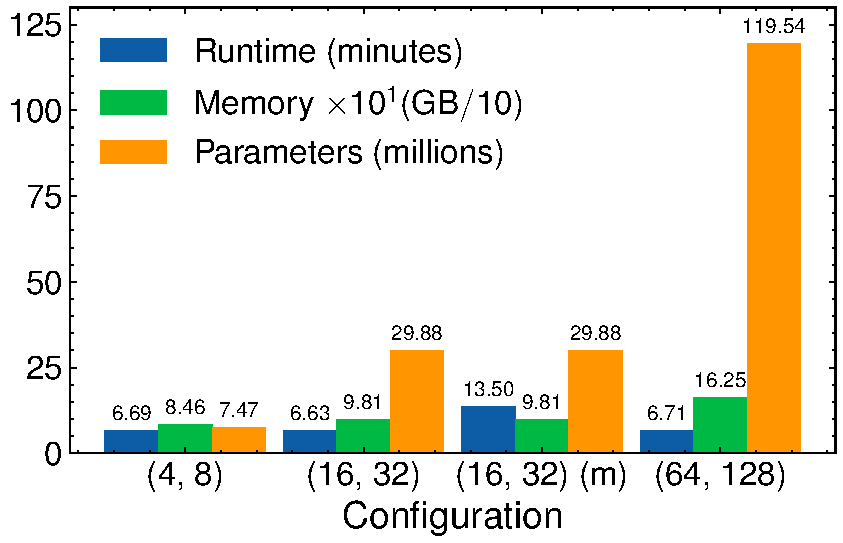
\includegraphics[width=0.9\linewidth]{../images/I.17 Results_A100_metrics.pdf}
        \caption{\emph{TrainingTime}, \emph{TrainingMemory} and number of trained parameters comparison.}
    \end{subfigure}
    \caption{Trade-offs between the specialized models and the multi-task model in terms of loss evolution, \emph{TrainingTime}, \emph{TrainingMemory}, and number of trained parameters. The (m) indicates the multi-task model. These experiments were conducted with a GPU A100 instance on \href{https://colab.research.google.com/}{Google Colab}. For \textbf{(I.17)}.}
    \label{fig:I.17-A100-results}
\end{figure}

% (I.18) Provide the complete code used for fine-tuning in the ZIP file, following the instructions in Section 3.6 (include the following files: project_part1_evaluate.py, project_part1_repair.py, project_part1_hint.py, project_part1_utils.py, project_part1_prompts.py, project_part2_evaluate.py, project_part2_assemble_dataset.py, and project_part2_finetuning.py).

%%%%%%%%%%%%%%%%%%%%%%%%%%%%%%%%%%%%%
\clearpage

\section*{Acknowledgements}
Week 10's slides and listed references.

%%%%%%%%%%%%%%%%%%%%%%%%%%%%%%%%%%%%%
\bibliographystyle{unsrt}
\bibliography{references}

%%%%%%%%%%%%%%%%%%%%%%%%%%%%%%%%%%%%%
\clearpage

\section{Appendix: (I.3) Results of Project Part\#1}\label{appendix:I3-results}

\begin{table}[H]
    \caption{Overall results for GPT-4o-mini and Phi-3-mini with the basic prompt to generate program repairs. For \textbf{(I.1)} and \textbf{(I.3)}.}
    \vspace{0.5\baselineskip}
    \centering
    \begin{tblr}{
        colspec = {|Q[c,m]|Q[c,m]|Q[c,m]|},
        colsep=4pt,
        vlines,
        hlines,
        hspan=minimal,
        vspan=center,
        row{1} = {font=\bfseries}
        }
        Model       & \textit{RPass} & \textit{REdit} \\
        \hline
        GPT-4o-mini & $88.0$         & $23.77$        \\
        Phi-3-mini  & $36.0$         & $18.11$        \\
    \end{tblr}
    \label{appendix-I3-results}
\end{table}

%%%%%%%%%%%%%%%%%%%%%%%%%%%%%%%%%%%%%
\clearpage

%%%%%%%%%%%%%%%%%%%%%%%%%%%%%%%%%%%%%
\end{document}

%%%%%%%%%%%%%%%%%%%%%%%%%%%%%%%%%%%%%
%%%%%%%%%%%%%%%%%%%%%%%%%%%%%%%%%%%%%